% =============================================================================
% Template dissertation using the qdissertation class
% =============================================================================
% This file is the main entry point. Build: make (uses latexmk; see Makefile).
% To use another engine: make ENGINE=xelatex or make ENGINE=lualatex.
%
% SPDX-FileCopyrightText: 2026 Frank Langbein <frank@langbein.org>
% SPDX-License-Identifier: LPPL-1.3c
% SPDX-License-Identifier: CC-BY-SA-4.0
%
% This template and other .tex/.bib files in this directory are part of the
% same work and may be distributed and/or modified under the LaTeX Project
% Public License (LPPL), version 1.3c. See LICENSE file.
%
% -----------------------------------------------------------------------------
% Overview (qdissertation class)
% -----------------------------------------------------------------------------
% The class is a wrapper around the standard book class. Layout: A4, 12pt,
% 3cm margins; single line spacing; ragged-right; main text 12pt, footnotes and
% captions at least 11pt; preliminary pages in roman numerals, then Arabic
% for main matter. Chapter style: top bar in header, ``Chapter N'' or
% ``Appendix A'' in header; number/letter and title on first line of chapter.
%
% -----------------------------------------------------------------------------
% Variations (degree, structure)
% -----------------------------------------------------------------------------
% Select your degree via \degree below; commented alternatives shown for
% BSc, MSc, MPhil. For some institutions, Chapter 6 (Reflection on Learning)
% may be omitted or merged into another chapter; comment out that \chapter
% and \input as needed.
%
% -----------------------------------------------------------------------------
% Class options
% -----------------------------------------------------------------------------
% Font: mixed (default) = sans text + serif math; sans = all sans-serif;
%   serif = serif text and math.
% Layout: oneside (default) or twoside.
% Citation: numeric (default) = plainnat, [1], [1,2]; harvard = agsm, (Author, 2000).
% Line spacing: single (default); onehalfspacing; or linespread115/linespread12
%   for institutions allowing 1.0--1.3.
% Engine: pdfTeX vs XeLaTeX/LuaLaTeX is detected for font setup.
%
% -----------------------------------------------------------------------------
% Metadata and title page
% -----------------------------------------------------------------------------
% \title, \author, \degree, \university, \date drive the generated title page.
%
% -----------------------------------------------------------------------------
% License and copyright (SPDX)
% -----------------------------------------------------------------------------
% \copyrightholder defaults to \author; \licenseyear defaults to current year.
% When \license is set: (1) a copyright page is inserted after the abstract;
% (2) a License chapter is inserted just before the bibliography.
% If qdissertation-licenses.tex is present, the class loads it for full
% license text; otherwise name + URL only.
%
% -----------------------------------------------------------------------------
% Float placement (figures, tables, algorithms)
% -----------------------------------------------------------------------------
% Placement letters: h = here, t = top, b = bottom, p = float page. E.g.\@
% [htbp], [t], [!t]. Use [H] (float pkg) sparingly. The class relaxes float
% parameters so more floats fit per page.
%
% -----------------------------------------------------------------------------
% LaTeX formatting: \citep/\citet (not \cite); ~ before \citep/\citet after a word;
% \@ after abbreviation; ~ for non-breaking (Fig.~1); -- en-dash, --- em-dash.
% Reviewer comments: %ID (e.g.\@ %F) at line start, space after ID.
%
% -----------------------------------------------------------------------------
% Word count: run ``make wordcount'' (texcount -inc; per-file and total with
% caption words shown separately so you can apply your institution's rules).
% Word limits typically apply to main body only; exclude front matter, captions,
% appendices. Confirm your institution's word limits and structure before submission.
%
% -----------------------------------------------------------------------------
% Submission: ensure PDF has embedded fonts (pdflatex does this by default),
% no encryption, and is compatible with your institution's requirements.
% Run make wordcount and confirm main-body limit. Appendices and captions
% are excluded from word counts in many institutional rules.
% =============================================================================
\documentclass[mixed,oneside,numeric]{qdissertation}

% -----------------------------------------------------------------------------
% Optional: use a different acronyms file
% -----------------------------------------------------------------------------
%\renewcommand{\qdissertationacronymfile}{my-acronyms.tex}

% -----------------------------------------------------------------------------
% Useful packages for dissertation writing
% -----------------------------------------------------------------------------

% Tables
\usepackage{tabularray}      % Flexible column types, rules, longtblr for multi-page tables
\usepackage{longtable}       % Tables that span multiple pages (or use tabularray longtblr)

% Math, symbols, related
\usepackage{mathtools}       % Extensions to amsmath (matrix envs, \DeclarePairedDelimiter)
\usepackage{pifont}          % Dingbat symbols, e.g. \ding{51}, \ding{43}
\usepackage{siunitx}         % Units and numbers: \SI{3}{m/s}, \num{1000}
\usepackage{relsize}         % \textlarger, \textsmaller for relative font sizing
\usepackage[version=4]{mhchem} % Chemical formulae: \ce{H2O}, \ce{CO2}, \ce{^1H-NMR}

% Floats
\usepackage{float}           % [H] = here definitely
\usepackage{stfloats}       % Improved placement for bottom floats
\usepackage{subcaption}     % Subfigures with (a), (b) and per-subfigure captions
\usepackage{rotating}       % \begin{sidewaystable}, \begin{sidewaysfigure} for wide content

% Algorithms
\usepackage{algorithm}       % Numbered algorithm floats and List of Algorithms
\usepackage[noend]{algpseudocode}

% Other useful packages
\usepackage{lipsum}          % Placeholder text: \lipsum[n], \lipsum[1-5], etc.
\usepackage{enumitem}       % Customise list labels, spacing
\usepackage{verbatim}       % \begin{verbatim} ... \end{verbatim} for code
\usepackage{afterpage}      % \afterpage{\clearpage} to clear after current page

% -----------------------------------------------------------------------------
% Dissertation metadata
% -----------------------------------------------------------------------------
\title{Template Dissertation Title: Each Word Capitalised}
\author{Your Full Name}
% Degree
\degree{BSc Computer Science}
% \degree{MSc Advanced Computer Science}
\university{Your University}
\date{February 2026}

% License and copyright following SPDX. (optional; comment out if not needed).
% Needs qdissertation-licenses.tex for license text in the License chapter.
\license{CC-BY-SA-4.0}
\copyrightholder{Your Full Name}
\licenseyear{2026}

\begin{document}

\frontmatter

% \maketitle{...} produces: title page, (copyright page if \license set), abstract,
% then frontlists: TOC, List of Figures, List of Tables, List of Algorithms,
% List of Acronyms (if acronyms.tex defines \newacronym).
% Current order: Title, (copyright), Abstract, TOC/LOF/LOT/LOA, Dedication,
% Acknowledgements. Some institutions prefer Acknowledgements before TOC;
% reordering is optional and project-specific.
% Typically 200--300 words. State problem, methods, and main results.
\maketitle{%
  This is the abstract: a short, self-contained summary of the dissertation.
  It should state the problem, methods, and main results so that a reader
  can understand the scope without reading the full document. Replace with
  your own abstract.
}

% -----------------------------------------------------------------------------
% Optional front-matter chapters (unnumbered)
% -----------------------------------------------------------------------------

\chapter{Dedication}
% Replace with your dedication (one or two lines).
To my family.

\chapter{Acknowledgements}
% Replace with your acknowledgements. Here you can also acknowledge any contributions from other
% parties to the work.
I thank my supervisors and colleagues for their support.

%\chapter{Declaration}
% Replace with your declaration (e.g. that the work is your own, and any
% required statements on collaboration, publications, or word count).
% Often this is submitted in separate forms or not needed, and does not
% have to be here.
%This dissertation is the result of my own work. Where reference is made to other work, this is indicated in the text.

%\chapter{Publications, data and code}
\chapter{Data and code}
% List publications, if available or maybe planned, and state where data and code produced for this
% dissertation are available. Note, you usually must submit any sources and simlar you ahve
% written with your dissertation.
% Replace with your own entries; you can use \citep{key} for publications.

%\section{Publications}
% Papers (and optionally other outputs) that form part of or arise from this thesis.
% These can also be discussed in the introduction (what has been published or is planned).
%\begin{enumerate}
%  \item Author. Title. \textit{Journal}, volume, pages, year.~\citep{example-paper}
%\end{enumerate}

\section{Data}
% Datasets produced in this work and where they are available (repository, DOI, or ``on request'').
Data supporting this dissertation are available from [repository/DOI or ``available on request'']. Replace with your statement.

\section{Code}
% Software or code produced in this work and where it is available (repository, DOI, etc.).
Code produced for this dissertation is available from [repository/DOI or ``available on request'']. Replace with your statement.

\mainmatter

% -----------------------------------------------------------------------------
% Main chapters: standard dissertation structure
% -----------------------------------------------------------------------------
% For some institutions, Chapter 6 (Reflection on Learning) may be omitted or
% merged; comment out the \chapter and \input for C6 as needed.
\chapter{Introduction}\label{ch1}
% =============================================================================
% CHAPTER 1: Introduction
% =============================================================================
% SPDX-FileCopyrightText: 2026 Frank Langbein <frank@langbein.org>
% SPDX-License-Identifier: LPPL-1.3c
%
% Suggested sections: Motivation and context; Aims and objectives; Contributions;
% Dissertation structure (roadmap). Optional: Scope (boundaries of the work),
% Terminology or key terms. Start with a short chapter intro (no \section) before
% the first section. This file also demonstrates template features; see
% Section~\ref{sec:ch1-reference}. Remove that section for your own report.
% =============================================================================

% -----------------------------------------------------------------------------
% Chapter intro (no section): one short paragraph before the first \section
% -----------------------------------------------------------------------------
\newthought{Media Players} are devices that focus on the delivery of music files, predominantly for leisure. Having a fondness for music, the Author aimed to make the playback of music as accessible as possible for the cognitively impaired. This project has a particular focus on patients with dementia, an umbrella term of diseases that impact cognitive ability.

% -----------------------------------------------------------------------------
% Motivation and context (typical first section)
% -----------------------------------------------------------------------------
% Use \section, \subsection, \label{key}. Refer with \ref{key} or \autoref{key}.
\section{Motivation and context}\label{sec:motivation}
Dementia is a syndrome that the Author has had experience with before through meeting an extended family member. Seeing the gravity of the mental degradation that can occur, when the Author saw the opportunity to develop a solution for the betterment of the 'quality of life' for these patients, they immediately expressed interest. Being the first project the Author has done in the field of accessibility, the Author had much to learn and they were excited to do so.

Doing preliminary research into media players, there did exist tailored devices for the patients with dementia on the market already but none of these contained any form of remote management, which was a gap in the market the Author decided to address.

% Aims and objectives (typical second section)
% -----------------------------------------------------------------------------
% Use \citep{} (parenthetical) or \citet{} (narrative), not \cite.

\section{Aims and objectives}\label{sec:objectives}
The aims and objectives of the project were as follows:
\begin{enumerate}
  \item Develop a tangible device that can be interacted with remotely which is able to play given media.
  \item Engage with social care researchers in a productive manner throughout the development of the device.
  \item Ensure the device is simple to use, lowering the barrier of entry for the device.
  \item Develop a secondary way of interaction with the device if time allows it.
\end{enumerate}

% -----------------------------------------------------------------------------
% Dissertation structure / roadmap (typical final section of introduction)
% -----------------------------------------------------------------------------

\section{Dissertation structure}\label{sec:roadmap}
The Dissertation you are about to read will have the following structure: 
\begin{itemize}
  \item \textbf{Chapter~\ref{ch2}} (Background): context, related work, problem statement.
  \item \textbf{Chapter~\ref{ch3}} (Methodology): research design, specification, system design, implementation.
  \item \textbf{Chapter~\ref{ch4}} (Results and Evaluation): setup, results, evaluation, limitations.
  \item \textbf{Chapter~\ref{ch5}} (Conclusions and Future Work): summary and next steps.
  \item \textbf{Chapter~\ref{ch6}} (Reflection on Learning): transferable learning.
  \item \textbf{Appendix~\ref{app:results}}: additional results.
\end{itemize}



\chapter{Background}\label{ch2}
% =============================================================================
% CHAPTER 2: Background
% =============================================================================
% SPDX-FileCopyrightText: 2026 Frank Langbein <frank@langbein.org>
% SPDX-License-Identifier: LPPL-1.3c
%
% Suggested sections: Context (or Wider context / Domain and context); Related
% work (or Literature review / Prior work); Problem statement (and research
% question(s)). Optional: Theory and concepts; Stakeholders and constraints
% (as subsections of Context or separate). End with a clear problem statement.
% Assume a competent reader; avoid lengthy descriptions of standard tools.
% =============================================================================
\newthought{Tackling a project} with a foothold into an industry the author had no prior stake in, background research was necessary. This ensured that the project remained novel but also did not try to re-invent anything that may already exist on the market. In this chapter, the wider context and related works are explored, informing the development of the proposed solution.

\section{Context}\label{sec:context}
% Wider context, domain, motivation. Optional subsections: stakeholders,
% constraints, assumptions.
Around half a million people suffer from dementia in the UK \citep{NHS2026}, a syndrome related to multitude of diseases including memory loss and degradation of mental faculties. This can cause confusion in executing everyday tasks, such as operating a music player. This resonated with the author who decided to undertake this project to understand the diseases, and help research accessible technologies to improve the quality of life of these patients.

\subsection{Technical Context}\label{subsec:tecContext}
The main stakeholders of the project were patients with dementia as the device was tailored towards their needs and what they would find easy to use. This was reflected in simplification of \gls{ui} elements \citep{10.1007/978-3-642-39473-7_39}. In this instance, the \gls{ui} has been replaced with physical buttons and tangible objects. This concept was later peer-reviewed by the experts over at ENRICH Cymru and the idea of simplicity was validated. 

The project's stakeholders wasn't limited to just these end users however, but the management staff that would be operating the device predominately. Stakeholders were extended to the carers of the dementia patients and the dementia patients' families, given their involvement in the operation of the proposed solution. 

Whilst the proposed solution aims to provide as much self-sufficiency to the patients as possible, it is unrealistic to assume that this would be possible for every patient in a given care home. Keeping the device simple to operate was paramount as nurses enlisted in the care of dementia patients reported having their schedule "destroyed" and having to reorganise their day, which ultimately took time from caring for these patients as they rarely cared for just dementia patients \citep{krupic2020experience}. The remote aspect of the proposed solution would also help save time, as support staff would not have to be physical present in the same room as the patient, allowing for them manage the device from anywhere within the care home.

The family of the patients would also have a stake in this project. Given the carers of these patients already had a lot on their plate, families could be a viable alternative for care, as the carers usually did not have access to extra personnel \citep{krupic2020experience}. Family members of the patients may have varying degree of tech literacy so simplicity and ease of operation is once again highlighted.

Given the time constraint of 12 weeks, it was unrealistic to include all features, so some constraints were put in place. An example of such was the omission of development of a graphical \gls{ui} for the remote management aspect, to save time for development of core features that were necessary for the functionality of the media player.

\subsection{Medical Context}\label{subsec:medContext}
Dementia as a disorder encompasses a variety of different 'neuropsychiatric symptoms' or \gls{bpsd} within its definition. These symptoms consist of disturbed emotions, mood, perception, thought, motor activity, and altered personality traits, as designated by the International Psychogeriatrics Association. All of these symptoms are associated with high levels of distress for the patients and their caregivers \citep{10.3389/fneur.2012.00073}.

The effects of dementia can also manifest themselves in the form of behavioural problems, being the main reason that caregivers end up placing their patients into nursing homes \citep{stoppe1999behavioural}. However, these problems are not universal and need to be taken on a case by case basis \citep{10.1001/jama.1982.03330030039022}. The treatment for these problems needs to be tailored towards the patient, which can be reflective on the type of music that they used to enjoy listening to as a form of musical therapy, which can be beneficial in the short-term \citep{mcdermott2013music}.

Patients with dementia, although experiencing diminished cognitive ability, still tend to retain a large portion of their musical ability, even in advanced stages of the syndrome \citep{BAIRD2015207}. This may range from playing a given instrument and recalling the accompanying musical theory \citep{beatty1988preserved} to recognition of familiar songs, acknowledging the presence of familiar lyrics and not responding to unfamiliar melodies \citep{cuddy2005music}. As this is a medium largely preserved in most cases of dementia, music may hold significance in the life of a dementia patient.

The positive impact of recreational activities for the "quality of life" for dementia patients can not be understated. As observed by A. S. Schreiner, E. Yamamota and H.Shiotani, patients with Alzheimer's dementia were able to \begin{quotation} express 'Happiness' over seven times more often during Recreation Time than during Ordinary Time
\end{quotation} concluding that all subject in their study exhibited 'Happiness' during recreation \citep{Schreiner01032005}. Although such importance has been recognised for recreation, most assistive technologies focused only on the 'ease of living' rather than the quality, showing a lack of development of technologies geared towards recreation \citep{10.1007/978-3-319-20916-6_38}. This provides a foundation and justification for the proposed solution. 

\section{Related work}\label{sec:related}
% Prior solutions, methods, or systems; identify gaps your work addresses.
% Optional subsections: by theme, chronology, or type (e.g.\@ systems, methods, theory).
Dementia-friendly media players are not a new technology. Following a similar ethos to the solution proposed, radios such as the "One Button Radio" and the "Relish Radio and Music Player" \citep{Danny2021} both do not feature a screen and only have buttons and dial controls with preset radio stations and playlists. The physical controls of these devices present themselves as a strength as operation is made as simple as possible, making independent operation easier and saving time for the caregiver as they need not be involved. These are examples of radios specifically designed for patients with dementia. It can be concluded that recreational devices geared towards the enjoyment of music for patients with impaired cognitive ability do exist but may lack in features, which may become more of a hindrance as development of newer technologies continues. This could be directly addressed by the proposed solution as features could be pushed remotely and would not need physical interaction to update.

Other devices on the market, not necessarily designed for patients with dementia, can also prove useful. The "Yoto Player 3rd Generation" was originally designed for children and is interfaced with cards that have been pre-programmed \citep{Yoto2023}. This device has then been adapted by MusicForDementia to include cards tailored to patients with dementia \citep{Utley2026}. This strongly implied that devices need not be designed specifically for the cognitively impaired, but would benefit from appropriate adjustment to cater towards their needs instead. The approach for the interface on this device largely inspired the tangible artefact interaction present on the proposed solution. The lack of an alternative however does present a learning curve that may be difficult for patients with dementia to overcome, mitigating inclusivity for different stages of the syndrome. The proposed solution tackles this by providing more than one way of interfacing with itself, allowing the patient with dementia to choose for themselves which control scheme suits them better.

Similarly, software-only solutions also exist. From MusicForDementia, m4dRADIO is a web application with preset buttons that tune into online radio stations that run 24/7 with the press of the button \citep{UtleyRadio2026}. This can be put onto a touch screen tablet, so the patient can tap onto the button and listen to music of their own volition. This form of media player can be seen as more accessible as specialist technology is not necessary; a device with a speaker and a web browser can prove just as useful. Utilising a general-purpose computing device provided a basis and proof of concept for adapting computers for accessible functionality, yet it highlights the need for customisation as each radio station is outside the caregivers control and runs the risk of being unsuitable for the patient that is being cared for. The proposed solution aims to address this by allowing complete control over the media being played out of the device.

A device tailored just for music playback may also be considered useful. \gls{dap}s are able to provide a simple experience for the end user, giving only the necessary controls to interact with the playback of the audio being played from them. The iPod Shuffle is a good example of this technology as it omits the use of a screen and favours simple controls over complicated \gls{ui}s. This is due to the focus on outputting audio, rather than creating a device that is a "jack of all trades" like the modern smartphone. Due to the variety on the market of \gls{dap}s, it is easier to source an unfitting device and may cause confusion with overcomplicated \gls{ui}s if sourced incorrectly. The proposed solution acts as a trusted device that aims to provide a similar service in a tailored manner.

Notably, none of these solutions allow for direct remote management, which is where this project comes into play. Most of these alternatives require physical interaction to amend music selection, adjust volume, and pause/play music. This project aims to eliminate this necessity.

\section{Problem statement}\label{sec:problem}
% Clear statement of the problem and, if applicable, research question(s).
Media Players for the cognitively impaired lack remote connectivity, allowing for ease of management through a local network. This project aims to create a media player that can be interfaced with remotely, physically and through tangible artifacts. The specific objectives of this project are as follows:
\begin{enumerate}
    \item Create a media player device that can output audio
    \item Develop a \textbf{physical} interface to interact with the media player
    \item Develop a \textbf{remote} interface to interact with the media player
    \item Develop a \textbf{tangible artifact} interface to interact with the media player
    \item Communicate with representatives of the stakeholders to retrieve feedback on the features and general operation of the device.
\end{enumerate}

Some assumptions about the user base were made to inform design decisions, these being:
\begin{itemize}
    \item The facility for the patients has access to a computer network.
    \item The facility has computers that are connected to the same network.
    \item The facility has access to a mouse, keyboard and monitor to perform the initial set-up on the device.
    \item The device is setup with assistance of a carer.
\end{itemize}
Rectifying these assumptions would be addressed if more time and resources were available, being further discussed in section \ref{sec:future}.


\chapter{Methodology}\label{ch3}
% =============================================================================
% CHAPTER 3: Methodology (or ``Specification, Design and Implementation'' / ``Approach'')
% =============================================================================
% SPDX-FileCopyrightText: 2026 Frank Langbein <frank@langbein.org>
% SPDX-License-Identifier: LPPL-1.3c
%
% This chapter describes how your solution works. Title it Methodology, Approach,
% or Specification, Design and Implementation; adapt or split as needed. Not all
% sections below apply to every project---pick, omit, or rename.
%
% Suggested sections by project type:
%   System design:  Specification, System design, Implementation. Optional: Datasets
%                   if data is central; Ethical considerations.
%   Research:       Research design, Literature and evidence (search strategy,
%                   inclusion criteria), Specification (= problem + requirements),
%                   Approach and solution, Implementation or experimental setup.
%   AI/ML:          Specification, Datasets, AI/ML models, System design (if a
%                   larger system), Implementation. Optional: Research design,
%                   Literature and evidence; Summary.
% =============================================================================

\newthought{As the proposed solution} of this project is not research-based, appropriate system design took place to keep structure during the development process and to provide quantifiable milestones, aiding in discussion within weekly meetings with the project supervisor.

\section{Specification}\label{sec:spec}
% System design: requirements (what the system must do; optional subsections: functional, non-functional). Research: problem and what is required of a solution.
As discussed in section \ref{sec:related}, it can be observed that each existing device on the market only utilises one input method, whereas the proposed solution needs to listen out for up to three. These methods of input were chosen due to their simple interfaces, the inputs being: terminal commands, physical button interaction and tangible artefact interaction. Simplicity in said input methods can be identified as follows:
\begin{itemize}
    \item The terminal commands are short words part of the English language that describe what they do and are expanded on further using the \texttt{help} command.
    \item The buttons execute one simple command each.
    \item The tangible artefacts require the user to physically tap them against the device, providing a simple physical action the end user needs to perform instead of learning a \gls{ui}.
\end{itemize} 

Before implementation could begin, identifying clear deliverables and subsequent efficiency guidelines had to occur. This was done through the generation of Functional and Non-functional Requirement. These were generated by breaking down what was absolutely necessary for the proposed solution to do and to which degree each of these actions efficiency is necessary.

\subsection{Functional requirements}\label{subsec:funcreq}
To ensure consistency between these modes of input and outlining clear deliverables, the following functional requirements were proposed:
\begin{enumerate}
    \item\label{req:playBtn} Pressing the play/pause button \textbf{must} play and pause the current song being played.
    \item\label{req:skipBtn} Pressing the skip button \textbf{must} skip the current song being played to the next song in the playlist.
    \item\label{req:remoteCon} The device \textbf{must} be able to be interfaced with remotely.
    \item\label{req:correctCommand} Sending commands over a remote terminal \textbf{must} perform the action that it has been assigned to do so.
    \item\label{req:NFCcorrect} Presenting a tangible artifact to the appropriate antenna \textbf{must} perform a playlist switch to a given playlist present on the artefact.
    \item\label{req:audioPlayback} The device \textbf{must} play audio through a predefined speaker.
    \item\label{req:usable} The device \textbf{must} always be in a usable state. 
\end{enumerate}
\subsection{Non-functional requirements}\label{subsec:nonfuncreq}
In a similar vein, the proposed solution needs to function in an efficient and safe manner. It is unreasonable to expect the end users to have to wait extended periods of time for actions to be performed, and potentially compromise their network with the proposed solution as the attacker's entry point. Therefore, the following non-functional requirements were also proposed:
\begin{enumerate}
    \item\label{req:remoteTime} Commands over the remote terminal should take \textbf{no longer than} 5 seconds to execute. Given the simple nature of the commands passed into the terminal, the expectation of response time will likely be instant, although expectations may vary \citep{shneiderman1984response}.  
    \item\label{req:remoteAuth} Users without authorisation should \textbf{not} be able to connect to the device remotely, ensuring the security of the device.
    \item\label{req:easeofuse} The device needs to be \textbf{intuitive} and easy to use.
    \item\label{req:startupTime} Start-up of the device should take \textbf{no longer than} 2 minutes. This is based off experience throughout development on the Raspberry Pi on its average boot times and what the author expects to be the average expectation for boot times.
    \item\label{req:NFCtolerance} The device should read a presented tangible artifact successfully in \textbf{no more than} 10 attempts. This provides a reasonable buffer identifying if the data collection delay is a hardware/software fault or due to user error.
    \item\label{req:scalability} The device should be \textbf{scalable}, and not suffer any performance drops as the playlists increase in size.
    \item\label{req:reboot} The device should \textbf{reboot} after a power cut and return to a \textbf{workable state} once power is restored.
\end{enumerate}

\section{AI and machine learning models}\label{sec:aiml}
% AI/ML: model choice, training and validation, evaluation methodology. Omit otherwise.
Although not instrumental to the design, AI chatbots powered by \gls{llm}s were utilised throughout the development of this project. These \gls{llm}s were used in a supportive capacity, largely through troubleshooting code or brainstorming ideas on how to execute potential features, in particular the utilisation of Python Sockets to execute terminal commands. Each piece of code produced by these models were thoroughly examined and rigorously tested to ensure it was efficient, no vulnerabilities were present and to further the understanding of the author as to what the code intends to do. The code was then rewritten and adapted to a particular use case.

The \gls{llm}s utilised for this project are the following:
\begin{itemize}
    \item Claude by Anthropic \citep{Anthropic2026}.
    \item Gemini by Google \citep{GoogleAI2026}.
    \item Microsoft Copilot by Microsoft AI and OpenAI \citep{MicrosoftAI2026}.
\end{itemize}

\section{System design}\label{sec:design}
% System design: architecture, data flow, behaviour (UML, ER, state charts). Use diagrams. Research: use ``Approach and solution'' for your proposed solution(s).
The system has been designed around three main hardware components:
\begin{enumerate}
    \item \texttt{Raspberry Pi 4 Model B}
    \item \texttt{Arduino Expansion Shield} acting as an Arduino Leonardo board
    \item \texttt{Bluetooth Speaker} in this case, a Google Nest Mini.
\end{enumerate}
However, the Raspberry Pi and Arduino Board are connected unconventionally, due to a GrovePi+ being already attached to the header pins of the Raspberry Pi. They are instead connected through a USB port on the Raspberry Pi itself. The Arduino is necessary here to connect the \gls{nfc} Reader Module, as its Base Shield possesses a UART connection, that the GrovePi+ does not have access to. A detailed diagram of how these components are connected with all accompanying sensors, buttons and speakers can be seen in Figure \ref{fig:sysoverH}.

\begin{figure}[H]
  \centering
  \fbox{\rule{0pt}{4cm}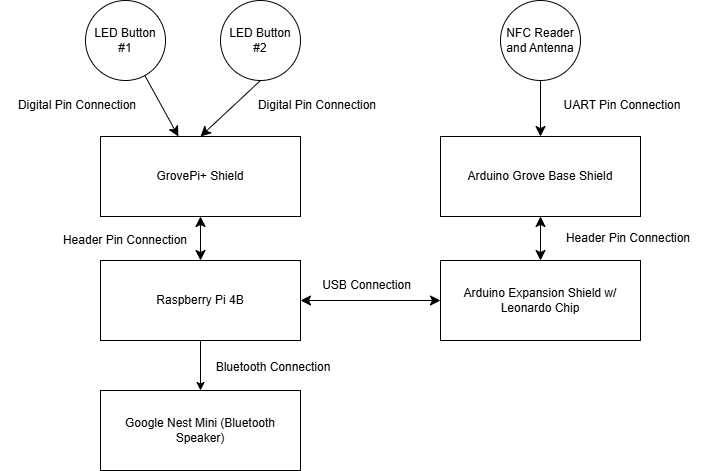
\includegraphics[width=0.97\textwidth]{images/SystemOverviewHardware}}
  \caption[System Overview - Hardware]{System Overview - Hardware}\label{fig:sysoverH}
\end{figure}

The software this project consists of can be separated into 3 main scripts:
\begin{enumerate}
    \item \texttt{client.py}, used for sending commands to the main program.
    \item \texttt{server.py}, housing the core functionality of the media player and receiving commands from both the Arduino and \texttt{client.py}.
    \item \texttt{reading\_nfc.ino}, used for reading the data off \gls{nfc} tags.
\end{enumerate}
This separation was necessary due to factors revolving around how UNIX sockets work between programs (necessitating the separation for communication to occur) and different systems requiring different programming languages (in this case, the Arduino running scripts in C++).  

An additional script for the Arduino also exists called "\texttt{writing\_nfc.ino}" but it is only necessary when creating new \gls{nfc} tags for new or existing playlists. A detailed diagram of how these interact with each other can be seen in Figure \ref{fig:sysoverS}.

\begin{figure}[H]
  \centering
  \fbox{\rule{0pt}{4cm}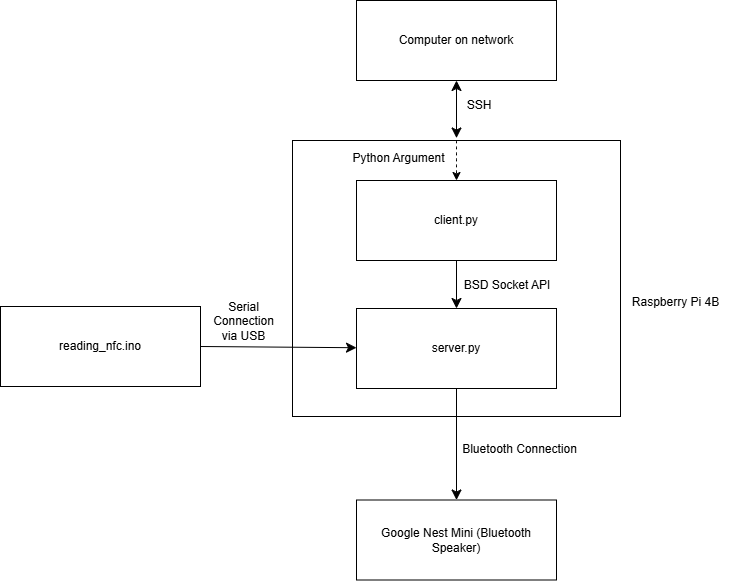
\includegraphics[width=0.97\textwidth]{images/SystemOverviewSoftware}}
  \caption[System Overview - Software]{System Overview - Software}\label{fig:sysoverS}
\end{figure}

The Python scrips utlises 2 external libraries to execute all of its functions, the rest being included in a Python 3 installation. The list of the libraries and what they were for is as follows:
\begin{itemize}
    \item grovepi, one of the external libraries that allows for direct interaction with the pins on the GrovePi+ shield.
    \item python-vlc, the other external library that allows for the music to be played through Raspbian's default media player VLC. Controls for the songs are managed through this library.
    \item time, a native Python library that introduced delays in the scripts, allowing for Bluetooth connection to occur without disruption.
    \item threading, a native Python library that allowed for multiple functions (in this case, reading \gls{nfc} tags and receiving terminal commands) to run concurrently.
    \item socket, a native Python library that utilises the BSD Socket API to communicate between \texttt{server.py} and \texttt{client.py}.
    \item subprocess, a native Python library that allowed for execution of terminal commands (in this case, bluetoothctl).
    \item os, a native Python library that read all of the song files in a given directory to construct a playlist.
    \item serial, a native Python library that facilitated reading from the serial port. 
    \item re, a native Python library that could enact regular expressions on the payloads of the \gls{nfc} tags.
    \item random, a native Python library that facilitated the "shuffle" functionality in the media player.
\end{itemize}

The C++ sketches for the Arduino utilised a library provided by Seeed Studios to interface with the \gls{nfc} reader, using \gls{ndef} formatting \citep{SeeedStudios2020}.

A full list of the hardware that was used in this project is the following:
\begin{itemize}
    \item \texttt{Raspberry Pi 4 Model B}
    \item \texttt{MicroSD Card 32Gb}
    \item \texttt{GrovePi+ Shield}
    \item \texttt{2 Grove LED Buttons}
    \item \texttt{Arduino Expansion Shield for Raspberry Pi B+ (V2.0)}
    \item \texttt{Grove Base Shield for Arduino}
    \item \texttt{Grove \gls{nfc} Reader}
    \item \texttt{5 \gls{nfc} tags}
    \item \texttt{Google Nest Mini}
    \item \texttt{Laptop} capable of \gls{ssh}
\end{itemize}

\section{Ethical considerations}\label{sec:ethics}
Dealing with a protected characteristic such as disability means ethics is rooted deeply within this project. To be able to user test with the stakeholders, full ethics approval is required. Given the timescale of this project, this was not feasible. 

The author instead opted to omit meeting the stakeholders directly, and in their stead, work with carers in the field instead. An argument can be made that since the author's intention was to communicate with private care homes with the assistance of ENRICH Cymru, simplified ethics could still be applied as they are not NHS staff.

For the sake of simplicity, the decision to include workers was also scrapped. Had more time and resources be allocated towards this project, researchers in the field would instead be the subject of user tests to hopefully provide actionable feedback on the proposed solution.

\section{Implementation}\label{sec:impl}
% Realisation: key implementation choices and critical code; avoid describing every module. Optional: tools, platform, problems encountered.
The goal of the implementation was to create each feature of the proposed solution one at a time, ensuring each feature worked in isolation before it was implemented to the system at large. The device was prepped with the prerequisites for working with the given peripherals and the following features were developed in order:
\begin{itemize}
    \item Button interaction was developed for the Grove LED Buttons.
    \item Music Player functionality was mapped to the buttons.
    \item Terminal interaction was developed through Python Sockets.
    \item Start-up behaviour was configured and scripts amended to accommodate it.
    \item \gls{nfc} interaction was developed on an Arduino and integrated into the system.
\end{itemize} 

\subsection{Initial Setup}\label{subsec:setup}
Producing a device that has been designed for mass rollout, a consistent and stable development environment was of paramount importance. It needed to be reproducible, so all units could have the same underlining technologies, and able to communicate with the modules used to interface with the device. To achieve this goal, all the appropriate libraries for the GrovePi library to work were installed on the most current image that supported the peripherals.

Incompatibilities throughout development helped inform this choice. They ranged from deprecated libraries within an older OS version, such as \texttt{easy\_install}, to the OS kernel itself and the underlying frameworks for communication over the \gls{i2c} interface \citep{IOTGarage2025}.

The GrovePi+ itself and its accompanying software and libraries helped identify each of these dependencies. Correct Raspberry Pi OS image choice went on to highlight the importance of the development environment as a whole, rather than in terms of package incompatibilities. This was largely due to the GrovePi+ also being a peripheral that has since been discontinued \citep{PiHut} so continued support from the manufacturer had ceased at the time of the development of the proposed solution.

The pre-configured image provided by Dexter Industries for the GoPiGo family of robots was considered as a potential candidate for the operating system \citep{DexterIndustriesGoPiGo2026} but after examining the image, it was not suitable for the use case, being bloated with unnecessary applications and local web server hosting that would waste system resources when running idle.

The importance of the open-source community helped drive the image choice as the kernel incompatibility \citep{cyclicalobsessive2024} and countless other nuances of other images (such as lacking appropriate public keys for \texttt{apt update} \citep{Jean2026} and outdated source lists in \texttt{/etc/apt/sources.list} \citep{rpdom2026}) were identified through community driven web-forums.

The decision to follow a guide provided by IOT Garage \citep{IOTGarage2025} and the installation of the \texttt{2024-10-22-raspios-bullseye} image was made, which is the current image on the proposed solution. This provided a compromise for currency of the image and having the appropriate OS kernel and \gls{i2c} communication framework. The only deviation from the guide is the copying of both the \texttt{di\_i2c} and \texttt{di\_mutex} modules (they both depend on each other) into the Python 3.9 directory.
\begin{fullwidthfigure}[H]
  \centering
  \fbox{\rule{0pt}{2cm}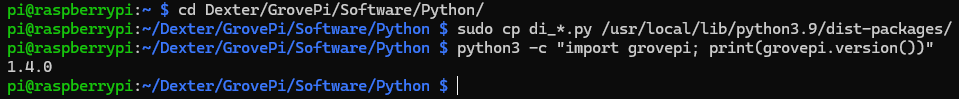
\includegraphics[width=0.97\linewidth]{images/workinggpi}}
  \caption[Movement of Modules and Test grovepi call]{Movement of Modules and Test grovepi call}\label{fig:workinggpi}
\end{fullwidthfigure}

The initial setup was now complete and development of the solution could commence. Although time-consuming, the initial setup helped highlight the idiosyncrasies of working on embedded systems. In a final system, working with peripherals that interfaced directly with the Raspberry Pi's \gls{gpio} pins would be prioritised instead. This would mitigate software dependencies as no third-party libraries would be necessary for interfacing with all of the peripherals, as the core library \texttt{GPIOZero} comes pre-installed on the latest Raspberry Pi Images \citep{bennuttal2024}. 

\subsection{Button Interaction}\label{subsec:btnint}
The proposed solution's main form of interaction is that of button presses on the Raspberry Pi. Once the GrovePi library was installed, focus was put on ensuring that button presses were recognised by the main Python script, using the GrovePi library.

Many of the Grove peripherals contained 2 ports in terms of addressing them and their properties. Working with these peripherals helped highlight how each proprietary module may have its own numbering convention on which port is assigned to what attribute of the peripheral. This was pivotal in the case of the Grove LED buttons where the addressing of the inputs was \textbf{offset by 1}. This was identified through the testing of the original port number and introducing the offset in algorithm \ref{alg:goodBtnTest}.

\begin{algorithm}[H]
    \caption{Successful Button Port Test - Python}
    \label{alg:goodBtnTest}
    \begin{lstlisting}[language=Python]
    import time
    import grovepi

    buttonP_pin = 3 # Port number + 1 recognises button input
    buttonS_pin = 8

    grovepi.pinMode(buttonP_pin, "INPUT")
    grovepi.pinMode(buttonS_pin, "INPUT")

    print("Ready!")
    \end{lstlisting}
\end{algorithm}
The offset identified was counterintuitive, as the labeling on the GrovePi+ shield was sequential, but the address for the button input was one higher. This quirk was not accurately described in the documentation provided the manufacturer and could cause potential issues with peripherals connected sequentially. 

\subsection{Music Player Functionality}\label{subsec:playlist}
Once the button presses were being recognised, music player functionality was implemented. This would include mapping button presses to their appropriate actions and loading a scalable playlist with a series of music files, with the possibility to shuffle them.

The python-vlc package was installed to interface with VLC, which acted as the media player for the proposed solution. It was chosen due to its universality of outputting various media files and open-source nature. Adaptations were made to the main script to map python-vlc's functions to the appropriate button presses, present in Algorithms \ref{alg:initVLC} and \ref{alg:mappedBtnPress}.

\begin{algorithm}[H]
  \caption{Initialisation of VLC Playlist - Python}
  \label{alg:initVLC}
  \begin{lstlisting}[language=Python]
    media_player = vlc.MediaListPlayer() # Intialises Playlist
    instance = vlc.Instance() # Creates VLC instance

    playlist = instance.media_list_new()

    for sound in os.listdir("AudioTracks"): # Creates a Playlist for all audio tracks in /AudioTracks/
        media = instance.media_new(f'AudioTracks/{sound}')
        playlist.add_media(media)

    media_player.set_media_list(playlist)
  \end{lstlisting}
\end{algorithm}
The MediaListPlayer here abstracts the entirety of the indexing of the music files, opting for a 'Black Box' solution, where each song within the \texttt{media\_list} is a separate object that cannot be interacted with directly. Instead, methods provided by python-vlc have to be utilised, as seen in algorithm \ref{alg:mappedBtnPress}.

\begin{algorithm}[H]
  \caption{Mapped Button Presses - Python}
  \label{alg:mappedBtnPress}
  \begin{lstlisting}[language=Python]
    buttonS_was_pressed = False
    buttonP_was_pressed = False
    while True:
        buttonP_state = grovepi.digitalRead(buttonP_pin)
        buttonS_state = grovepi.digitalRead(buttonS_pin)
        
        if buttonP_state == 0 and not buttonP_was_pressed:
            media_player.pause()
            buttonP_was_pressed = True
            
        if buttonS_state == 0 and not buttonS_was_pressed:
            media_player.next()
            buttonS_was_pressed = True
            
        if buttonS_state == 1 and buttonS_was_pressed:
            buttonS_was_pressed = False  
        elif buttonP_state == 1 and buttonP_was_pressed:
            buttonP_was_pressed = False

        time.sleep(0.05)
  \end{lstlisting}
\end{algorithm}
Interestingly, separate pause and play logic was not necessary to implement as the \texttt{vlc.MediaListPlayer} pause function acts as a toggle and pauses or plays respective of the current state of the player. The buttons actions have now been mapped with their designated actions.

To adjust for scalability and the implementation of more than one playlist, the function responsible for this was moved into a dedicated Python function. This was done for modularity and avoiding repeating code when a playlist is to be switched. It takes two arguments, the playlist name and a shuffle boolean. If shuffle is not passed, it defaults to False. The code snippet can be seen in Algorithm \ref{alg:loadplaylist}.
\begin{algorithm}[H]
  \caption{load\_playlist() - Python}
  \label{alg:loadplaylist}
  \begin{lstlisting}[language=Python]
    def loadplaylist(playlistName, shuffle="false"):
        if playlistName == '':
            return False
        
        try:
            os.listdir(f'AudioTracks/{playlistName}')
        except FileNotFoundError:
            return False
        
        playlist = instance.media_list_new()
        
        if shuffle.lower() == "true":
            songs = os.listdir(f'AudioTracks/{playlistName}')
            random.shuffle(songs)
            for sound in songs:
                print(sound)
                media = instance.media_new(f'AudioTracks/{playlistName}/{sound}')
                playlist.add_media(media)
        else:
            for sound in sorted(os.listdir(f'AudioTracks/{playlistName}')):
                print(sound)
                media = instance.media_new(f'AudioTracks/{playlistName}/{sound}')
                playlist.add_media(media)
        media_player.set_media_list(playlist)
        return True
  \end{lstlisting}
\end{algorithm}
This function is able to discern between valid inputs and returns either a True if a playlist switch has successfully occured or a False if an error was caught (either through the playlist not existing or a null value being inputted). This provides a lightweight version of error checking that helped streamline the testing process, as seen in algorithm \ref{alg:playlistTest}. 

This section helped illustrate the importance of reading documentation of an external library and how its dedicated data structures could be interfaced with.
\subsection{Terminal Interaction}\label{subsec:terminal}
% % GOAL
% Create terminal solution that can be interfaced using SSH
% % APPROACH
% UNIX Socket with client/server model
% % KEY DECISIONS/FINDINGS
% systemd gives no terminal

Remote Management was one of the key aims for this project and without the presence of a GUI to facilite this requirement, terminal commands were introduced. The approach taken for terminal interaction was utilising Python's \texttt{socket} library, creating a socket network architecture. 

The "remote" aspect for the Remote Management came from connecting to the device using \gls{ssh} and interfacing with the terminal provided from the connection, as example of such can be seen in Figure \ref{fig:sshEg}. \gls{ssh} was chosen as the remote solution as it is lightweight on a system, with the OpenSSH server not visibly impacting performance, and due to its security, requiring a key exchange at initial connection and credentials for each login attempt. Alternatives for remote management were also explored, such as \gls{vnc} with a desktop environment but a terminal window is still required.

\begin{fullwidthfigure}[H]
  \centering
  \fbox{\rule{0pt}{1.3cm}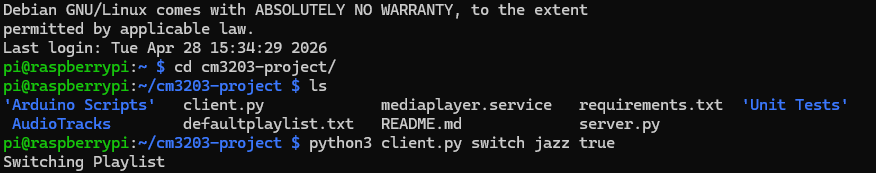
\includegraphics[width=0.97\linewidth]{images/sshExample}}
  \caption[SSH Example]{SSH Example - Switching Playlists}\label{fig:sshEg}
\end{fullwidthfigure}

Given the development context of the proposed solution, where \texttt{systemd} is utilised for running the main script on start-up, the socket architecture was chosen to send and receive commands via Python files, allowing for any \gls{ssh} session and terminal to interface with the device. A simpler approach was originally setup through the use of a \texttt{While True} loop executing in tandem with the button recognition commands, using the \texttt{threading} library, but the lack of an attached terminal ruled out this approach. Anthropic's \gls{llm} Claude was able to assist here, originally suggesting the utilisation of sockets, which it later drafted an implementation for \citep{AnthropicMarch2026}. 

The commands the user has at their disposal are:
\begin{itemize}
    \item play/pause, represented as "p"
    \item skip, represented as "s"
    \item switch, allowing the user to switch to the playlist passed as an argument
    \item help, providing a menu on what each command does 
\end{itemize}

Using a UNIX socket, a secondary smaller script \texttt{client.py} would send a message to \texttt{main.py} (now being renamed \texttt{client.py}) to decode and execute the command the message contained. The socket receiver now also needed to run in tandem, so it became the 2\textsuperscript{nd} thread and was executed using the \texttt{threading} library.

The 2 Python facilitating the communication over the socket architecture \texttt{client.py} and \texttt{server.py} can be seen in Algorithms \ref{alg:clientpy} and \ref{alg:socketReceiverSnip}.
\begin{algorithm}[H]
  \caption{client.py - Python}
  \label{alg:clientpy}
  \begin{lstlisting}[language=Python]
    import socket
    import sys

    def send_command(command):
        if command == '':
            return "Invalid command\n"
        
        socket_path = '/tmp/musicplayer.sock'
        client = socket.socket(socket.AF_UNIX, socket.SOCK_STREAM)
        client.connect(socket_path)
        
        client.send(command.encode())
        response = client.recv(1024).decode()
        client.close()
        return response

    if __name__ == '__main__':
        command = ' '.join(sys.argv[1:])
        response = send_command(command)
        print(response)
  \end{lstlisting}
\end{algorithm}
\texttt{client.py} takes the arguments that have been passed alongside its execution and encodes them to send over the UNIX socket. The response is limited to 1024 bytes due to them being simple enough, anymore would be unnecessary. This can be easily amended should more complex functionality be implemented.

\begin{algorithm}[H]
  \caption{terminal\_server() Snippet - Python}
  \label{alg:socketReceiverSnip}
  \begin{lstlisting}[language=Python]
    def terminal_server():
        server = socket.socket(socket.AF_UNIX, socket.SOCK_STREAM)
        socket_path = '/tmp/musicplayer.sock'
        if os.path.exists(socket_path):
            os.remove(socket_path)
        server.bind(socket_path)
        server.listen(1) # Listens out to only one command  
        while True:
            conn, _ = server.accept()
            data = conn.recv(1024).decode().strip()
  \end{lstlisting}
\end{algorithm}
To ensure that the clean-up process has been executed, \texttt{terminal\_server()} checks if the socket path already exists and deletes it if it remains. This ensures that the current socket has not impacted by previous commands that may have been passed prior to the execution of \texttt{client.py}.

The device could now receive terminal commands through any \gls{ssh} terminal. This section was able to bring light to how two separate Python scripts are able to interact with each other, simulating a network connection through the use of Python's \texttt{socket} library.
\subsection{Start-up Behaviour}\label{subsec:startup}
The device should not need remote interaction on start-up. If this was to be omitted, this would overcomplicate the device and make it inferior to devices already on the market, where simplicity thrives. Remote Management should be an add-on, rather than a necessary tool. The device therefore needed to start playing music the moment it turns on, or reboots after a power cut. This was done through the use of \texttt{systemd} on the Raspberry Pi, where a service was created that would run \texttt{server.py}.

Algorithm \ref{alg:playerServ} shows how \texttt{mediaplayer.service} file utilised in \texttt{systemd}. This service was moved to \texttt{/etc/systemd/system/} and activated using \texttt{systemctl start mediaplayer.service} resulting in it being executed each time the Raspberry Pi reboots. 
\begin{algorithm}[H]
  \caption{mediaplayer.service}
  \label{alg:playerServ}
  \begin{lstlisting}
    [Unit]
    Description=Music Player
    After=network.target sound.target

    [Service]
    ExecStart=/usr/bin/python3 /home/pi/cm3203-project/server.py
    WorkingDirectory=/home/pi/cm3203-project
    User=pi
    Environment=XDG_RUNTIME_DIR=/run/user/1000
    Restart=on-failure
    RestartSec=5

    [Install]
    WantedBy=multi-user.target
  \end{lstlisting}
\end{algorithm}
The utilisation of \texttt{Environment=XDG\_RUNTIME\_DIR=/run/user/1000} here ensures that the user has logged on, which happens automatically on start-up. It specifically double checks if the user session buffer has been created, ensuring VLC and PulseAudio are running, which \texttt{client.py} is dependent on. 

As the device utilises a Bluetooth speaker to play the desired media, the Bluetooth device needed to be paired on start-up as well. This was ensured through a function in \texttt{server.py} that executes before the main script does. It attempts to connect to a given MAC address of a Bluetooth device a total of 10 times, before it times out. This time-out then allowed for support to be carried out by a carer to connect a Bluetooth device manually. 

To ensure that some music is also played on start-up, the \texttt{load\_playlist()} function was called with a text file called \texttt{defaultplaylist.txt} that the end user is free to amend to a different playlist.

This section demonstrated how modern Linux systems execute programs on start-up through \texttt{systemd} through the utilisation of \texttt{.service} files.
\subsection{NFC Reading and Command Execution}\label{subsec:NFC}
As time allowed during the development of this project, tangible item interaction utilising \gls{nfc} was implemented alongside the button interaction. This was done through connecting the Raspberry Pi and an Arduino with the \gls{nfc} module attached to a \gls{uart} connection. These two devices were then connected over a USB, with the Raspberry Pi reading the output from the serial port of the USB bus.

The Arduino had two sketches, one for writing to the \gls{nfc} tags (Algorithm \ref{alg:writeNFC}) and one for reading them (Algorithm \ref{alg:readNFC}). Both scripts were adapted from sketches provided from the IOT Garage Lab Book GitLab \citep{Perera2024} and included a library to be able to interface with the module on the Arduino \citep{SeeedStudios2020}.

\begin{algorithm}[H]
  \caption{writing\_nfc.ino - C++}
  \label{alg:writeNFC}
  \begin{lstlisting}[language=C++]
    #include <NfcAdapter.h>
    #include <PN532/PN532_HSU/PN532_HSU.h>

    PN532_HSU pn532hsu(Serial1);
    NfcAdapter nfc(pn532hsu);

    String record_entry = "NAME_OF_PLAYLIST";

    void setup() {
        Serial.begin(9600);
        while(!Serial);
        Serial.println("NDEF Writer");
        nfc.begin();
    }

    void loop() {
        if (nfc.tagPresent()) {
            Serial.println("NFC TAG FOUND");
            NdefMessage message = NdefMessage();

            message.addUriRecord(record_entry);

            bool success = nfc.write(message);
            
            if (success) {
                Serial.println("Write succeeded.");
            } else {
                Serial.println("Write failed.");
            }
        }
    }
  \end{lstlisting}
\end{algorithm}

\begin{algorithm}[H]
  \caption{reading\_nfc.ino - C++}
  \label{alg:readNFC}
  \begin{lstlisting}[language=C++]
    #include <NfcAdapter.h>
    #include <PN532/PN532_HSU/PN532_HSU.h>

    PN532_HSU pn532hsu(Serial1);
    NfcAdapter nfc(pn532hsu);

    void setup() {
        Serial.begin(9600);
        while(!Serial);
        Serial.println("NDEF Reader");
        nfc.begin();
    }

    void loop() {
        if (nfc.tagPresent()) {
            NfcTag tag = nfc.read();
            tag.print(); // Prints to serial port
        }
        delay(1000);
    }
  \end{lstlisting}
\end{algorithm}

Once the tags have been written and been presented to the \gls{nfc} module, \texttt{server.py} extracted the information using Regular Expressions from the serial output of the USB bus, located through executing \texttt{ls} in \texttt{/dev/} \citep{Quibits2026}, and switches playlists based off the payload passed on the \gls{nfc} tag, as seen in Algorithm \ref{alg:readNFCPy}.

\begin{algorithm}[H]
  \caption{nfc\_reader\_switch() - Python}
  \label{alg:readNFCPy}
  \begin{lstlisting}[language=Python]
    #Accepting NFC Tags
    serial_port = '/dev/ttyACM0'
    baud_rate = 9600

    ser = serial.Serial(serial_port, baud_rate)
   
    while True:
        serData = ser.readline().decode('utf-8', errors='ignore')
        if serData.startswith("    Payload"):
            if serData.startswith("    Payload L") == False:
                print(serData)
                pattern = r'\.([a-zA-Z]+(?:\s+[a-zA-Z]+)?)'
                message = re.findall(pattern, serData) 
                if len(message) == 0:
                    print('Error reading NFC tag, attempt again...')
                else:
                    split_msg = message[0].split()
                    media_player.stop()
                    if len(split_msg) > 1:
                        loadplaylist(split_msg[0], split_msg[1])
                    else:
                        loadplaylist(message[0])
                    media_player.play()

  \end{lstlisting}
\end{algorithm}
The regular expression here extracts exactly the information that is needed from the NFC tag, given its formatting. Most of the data provided by scanning the NFC tag is unnecessary for the application for the proposed solution, so is omitted through checking for the desired line that carries the payload.

This section demonstrated how two separate embedded systems are able to communicate with each other, using a common interface as an intermediary (in this case, the serial port).

\section{Summary}\label{sec:summary}
% Optional: short summary of the methodology. Omit if the chapter is already concise.
The methodology for this project aimed to tackle each feature individually on a weekly basis, as proposed by the initial project plan. These features were:
\begin{enumerate}
    \item Set up the Raspberry Pi with GrovePi and all the necessary libraries.
    \item Implement button interaction so Raspberry Pi recognises input.
    \item Implement media player functionality with buttons and terminal interaction.
    \item Set up start-up behaviour so music player plays automatically.
    \item Implemenet \gls{nfc} interaction to switch playlists.
\end{enumerate}
This methodology remained fluid throughout development as no strict deadlines were imposed for the creation of these features. The methodology will be discussed more in depth in section \ref{sec:discussion}.

\chapter{Results and Evaluation}\label{ch4}
% =============================================================================
% CHAPTER 4: Results and Evaluation
% =============================================================================
% SPDX-FileCopyrightText: 2026 Frank Langbein <frank@langbein.org>
% SPDX-License-Identifier: LPPL-1.3c
%
% Suggested sections: Setup (or Evaluation setup / Experimental setup); Results;
% Discussion (or Evaluation and discussion); Limitations. Optional: Ablation
% studies (AI/ML); Comparison with baselines; Threats to validity. Describe how
% you demonstrated the system or hypothesis; include critical tests/experiments;
% critically appraise strengths and weaknesses.
% =============================================================================

\newthought{Tests within a system design project} are inevitable, as they dictate if a project was successful in its aims and has met its requirements. This section will demonstrate what tests were designed for the solution, the results drawn from these tests and will provide an analysis of the project as a whole.

\section{Setup}\label{sec:setup}
% Evaluation setup: data, metrics, baselines, how experiments or tests were run.
% Optional subsections: environment, hyperparameters, evaluation protocol.
Being a combination of a physical device and a software solution, different types of testing had to occur to fully evaluate the performance and accuracy of the solution. The testing conducted was a combination of unit testing and system testing. 

Unit testing was utilised for the modules that can be tested automatically using the \texttt{unit\_test} module in Python. These unit tests can be seen in Algorithms \ref{alg:socketTest} and \ref{alg:playlistTest}. These unit tests also ensured that the shuffle function was called to test if shuffle was passed, the playlist was in fact shuffled.

\begin{algorithm}[!h]
  \caption{socketCommand\_Test - Python}
  \label{alg:socketTest}
  \begin{lstlisting}[language=Python]
    import socket
    import client
    import unittest
    import time
    from unittest.mock import patch

    '''For this unit test, server.py needs to be running'''

    class Test_Socket_Commands(unittest.TestCase):
        def test_play(self):
            response = client.send_command('p')
            self.assertEqual(response, 'Paused/Resumed\n')
        
        def test_skip(self):
            response = client.send_command('s')
            self.assertEqual(response, "Skipped\n")
        
        def test_switch(self):
            response = client.send_command('switch default')
            self.assertEqual(response, "Switching Playlist\n")
            
        def test_invalid_switch(self):
            response = client.send_command('switch akjsdajkhsd')
            self.assertEqual(response, "Playlist not found\n")
            
        def test_help_command(self):
            response = client.send_command('help')
            self.assertTrue(response.startswith("'--------------\nhelp:"))
            
        def test_invalid_command(self):
            response = client.send_command('make sandwich')
            self.assertEqual(response, "Invalid command\n")
            
        def test_null_command(self):
            response = client.send_command('')
            self.assertEqual(response, "Invalid command\n")
            
        # Exit command to be tested manually as order of tests seems to execute exit command first
        # then the rest of the tests (resulting in failure)
  \end{lstlisting}
\end{algorithm}

\begin{algorithm}[!h]
  \caption{loadPlaylist\_Test - Python}
  \label{alg:playlistTest}
  \begin{lstlisting}[language=Python]
    import server
    import random
    import unittest
    from unittest.mock import patch

    class TestLoadPlaylist(unittest.TestCase):
        def test_valid_playlist(self):
            self.assertEqual(server.loadplaylist('default'), True)
            
        def test_invalid_playlist(self):
            self.assertEqual(server.loadplaylist('asjdasdajs'), False)
            
        def test_null_playlist(self):
            self.assertEqual(server.loadplaylist(''), False)
        
        @patch('random.shuffle')
        def test_shuffle_no_args(self, mock_shuffle):
            server.loadplaylist('default')
            self.assertFalse(mock_shuffle.called)
            
        @patch('random.shuffle')
        def test_shuffle_true(self, mock_shuffle):
            server.loadplaylist('default', 'true')
            self.assertTrue(mock_shuffle.called)
            
        @patch('random.shuffle')
        def test_shuffle_false(self, mock_shuffle):
            server.loadplaylist('default', 'false')
            self.assertFalse(mock_shuffle.called)
  \end{lstlisting}
\end{algorithm}
\clearpage

System tests were used for the hardware components of the proposed solution, in this case if the button presses are recognised and audio playing from the correct Bluetooth speaker. The system tests produce results that can be observed but require human interaction, hence why unit tests through Python's \texttt{unittest} module cannot be applied.

The baselines and acceptance criteria for these tests were derived from the functional and non-fuctional requirements, presented in section \ref{sec:spec}.

Testing of the \gls{nfc} module and its reliability was conducted through the use of amending the existing function, documenting:
\begin{itemize}
  \item How many attempts to scan a \gls{nfc} tag have been made.
  \item How many attempts were successful and switched playlists as intended.
\end{itemize}

This was done by creating counters in the form of a list (as they are mutable) that was updated throughout execution. For the function to gain access to these counters, they were passed as arguments and the appropriate \texttt{threading} call was amended to reflect this change. These amendedments can be seen in Algorithms \ref{alg:globalCounters}, \ref{alg:testNFCSwitch} and \ref{alg:NFCReaderCallAmend}.

\begin{algorithm}[!h]
  \caption{Counters for \gls{nfc} Test Snippet - Python}
  \label{alg:globalCounters}
  \begin{lstlisting}[language=Python]
    import time, grovepi, vlc, os, threading, socket, subprocess, serial, re, random

    buttonP_pin = 3 # For some odd reason, the port number + 1 recognises the appropriate button

    buttonS_pin = 8

    grovepi.pinMode(buttonP_pin, "INPUT")
    grovepi.pinMode(buttonS_pin, "INPUT")

    grovepi.digitalWrite(buttonP_pin - 1, 1)

    media_player = vlc.MediaListPlayer() # Intialises Playlist
    instance = vlc.Instance() # Creates VLC instance

    successfulNFCReads = [0] # New Addition
    attemptedNFCReads = [0]
  \end{lstlisting}
\end{algorithm}

\begin{algorithm}[!h]
  \caption{Amended nfc\_reader\_switch() with counter parameters - Python}
  \label{alg:testNFCSwitch}
  \begin{lstlisting}[language=Python]
    def nfc_reader_switch(successfulNFCReads, attemptedNFCReads): # Accetps new arguments
        #Accepting NFC Tags
        serial_port = '/dev/ttyACM0'
        baud_rate = 9600

        ser = serial.Serial(serial_port, baud_rate)

        while True:
            serData = ser.readline().decode('utf-8', errors='ignore')
            if serData.startswith("    Payload"):
                if serData.startswith("    Payload L") == False:
                    print(serData)
                    attemptedNFCReads[0] += 1 # Attempted read occured
                    message = re.findall(r'\.([a-zA-Z]+(?:\s+[a-zA-Z]+)?)', serData)
                    split_msg = message[0].split()
                    media_player.stop()
                    print(attemptedNFCReads)
                    if len(split_msg) == 0:
                        print('Error reading NFC tag, attempt again...')
                    else:
                        if len(split_msg) > 1:
                            loadplaylist(split_msg[0], split_msg[1])
                            successfulNFCReads[0] += 1 # If data extracted successfully, marked as successful
                        else:
                            loadplaylist(message[0])
                            successfulNFCReads[0] += 1
                    media_player.play()
  \end{lstlisting}
\end{algorithm}

\begin{algorithm}[!h]
  \caption{\texttt{threading} call amendment for \gls{nfc} Testing - Python}
  \label{alg:NFCReaderCallAmend}
  \begin{lstlisting}[language=Python]
    if __name__ == '__main__':
        threading2 = threading.Thread(target=nfc_reader_switch, args=(successfulNFCReads, attemptedNFCReads)) # Arguments passed into execution
        threading2.daemon = True
        threading2.start()
  \end{lstlisting}
\end{algorithm}
\newpage
Some preliminary logistical groundwork was also undertaken with the potential of user testing with care home staff with the assistance of ENRICH Cymru. This working relationship was established through visiting a conference with researchers in the field of care home, hosted by Stuart Allen, the project supervisor. Interest was expressed from ENRICH, however complications occurred during application for ethical approval. User testing therefore had to be abandoned for the project to continue ethically, as no response was given in time.
\section{Results}\label{sec:results}
% Main findings: present tables and figures; summarise key outcomes. Optional
% subsections: by research question, by dataset, or by metric.
The results of the test conducted for each component will be split up into corresponding sub-sections with their appropriate figures and test data. In summary, all of the unit tests and system tests passed. This was largely due to the testing spearheading development, encouraging error checking throughout to keep the system as reliable as possible.

\subsection{Terminal Command Testing Results}\label{subsec:terminalResults}
This module was evaluated using unit tests to see if the appropriate output was returned through the terminal. As seen in algorithm \ref{alg:socketTest}, each possible command bar the \texttt{exit} command has been set up as an automatic test, as the \texttt{exit} command was tested in isolation. Results of the tests are seen in Table \ref{tab:terminalResults}

\begin{table}[!h]
  \centering
  \caption{Terminal Commands Testing Table}
  \label{tab:terminalResults}
  \begin{tabularx}{\linewidth}{llXXl}
    \toprule
    Type of Testing Data & Input & Expected Output & Actual Output & Pass/Fail \\ \hline
    \midrule
    Normal & p & Song Paused & Song Paused & Pass \\ \hline
    Normal & s & Song Skipped & Song Skipped & Pass \\ \hline
    Normal & switch default & Switching Playlist & Switching Playlist & Pass \\ \hline
    Normal & switch default true & Switching Playlist & Switching Playlist & Pass \\ \hline
    Normal & exit & Exiting & Exiting & Pass \\ \hline
    Erroneous & x & Throws Error and prompts reinput & Throws Error and prompts reinput & Pass \\ \hline
    Erroneous & f & Throws Error and prompts reinput & Throws Error and prompts reinput & Pass \\ \hline
    Erroneous & switch asjdashd & Playlist not found & Playlist not found & Pass \\ \hline
    Null & N/A & Throws Error and prompts reinput & Throws Error and prompts reinput & Pass \\ \hline
    \bottomrule
  \end{tabularx}
\end{table}

All of the results returned a pass with handling all the types of data that could be passed into the terminal.
\clearpage
\subsection{Button Interaction Testing Results}\label{subsec:btnResults}
This module was evaluated using system tests as human input was necessary so automated unit tests were impractical to enact. The results for these tests can be seen in Table \ref{tab:buttonResults}.

\begin{table}[!h]
  \centering
  \caption{Button Interaction Testing Table}
  \label{tab:buttonResults}
  \begin{tabular}{lllll}
    \toprule
    Type of Testing Data & Input & Expected Output & Actual Output & Pass/Fail \\
    \midrule
    Normal & D2 button press & Song Paused & Song Paused & Pass \\
    Normal & D7 button press & Song Skipped & Song Skipped & Pass \\
    Erroneous & D3 button press & Nothing happens & Nothing happens & Pass \\
    Erroneous & D5 button press & Nothing happens & Nothing happens & Pass \\
    Null & N/A & Nothing happens & Nothing happens & Pass \\
    \bottomrule
  \end{tabular}
\end{table}
All of these system tests returned a pass with all of the documented button interactions, including inputs from mismatched port numbers. 

\subsection{Loading Playlist Testing Results}\label{subsec:playlistResults}
Being a self-contained function that did not require human interaction during its testing process, \texttt{load\_playist()} was a perfect candidate for the Python \texttt{unittest} module. The preconstructed unit tests attempts to load the \texttt{default} playlist with and without the \texttt{shuffle} parameter present. The results can be seen in Table \ref{tab:loadPlaylistTest}.
\begin{table}[!h]
  \centering
  \caption{load\_playlist() Testing Table}
  \label{tab:loadPlaylistTest}
  \begin{tabular}{lllll}
    \toprule
    Type of Testing Data & Input & Expected Output & Actual Output & Pass/Fail \\
    \midrule
    Normal & \texttt{default} & True & True & Pass \\
    Normal & \texttt{default} & Shuffle Not Called & Shuffle Not Called & Pass \\
    Normal & \texttt{default false} & Shuffle Not Called & Shuffle Not Called & Pass \\
    Normal & \texttt{default true} & Shuffle Called & Shuffle Called & Pass \\
    Erroneous & \texttt{asjdasdajs} & False & False & Pass \\
    Null & N/A & False & False & Pass \\
    \bottomrule
  \end{tabular}
\end{table}
All of the unit tests for this function were able to pass, demonstrating how the function is to behave. 
\subsection{NFC System Testing Results}\label{subsec:NFCResults}
The \gls{nfc} module also required human interaction during the testing process so was subject to system tests, instead of unit tests. The process of the test was to leave a \gls{nfc} tag onto the antenna for 100 cycles of scanning the tag and see what percentage scans were successful. The results of this test are visible in Table \ref{tab:NFCScanResults}
\clearpage
\begin{table}[!h]
  \centering
  \caption{\gls{nfc} Scan Robustness Testing Data}
  \label{tab:NFCScanResults}
  \begin{tabular}{llll}
    \toprule
    \gls{nfc} Tag Content & Attempted \gls{nfc} Scans & Successful \gls{nfc} Scans & Success Rate (\%)  \\
    \midrule
    \texttt{default} & 100 & 100 & 100\% \\
    \texttt{backrooms} & 100 & 100 & 100\% \\
    \texttt{jazz} & 100 & 100 & 100\% \\
    \bottomrule
  \end{tabular}
\end{table}

All of these preregistered \gls{nfc} tags were read at a 100\% success rate and enacted their appropriate playlist switch each time they were scanned.

\subsection{Response Time Testing Results}\label{subsec:execTimeResults}
Response Times for various components (including scalability of the playlists sizes) of the proposed solution were tested using either a stopwatch as execution occurred (in the case of time taken for the main script to be ran at boot, denoted by the predefined speaker playing the first song) or utilising the \texttt{time} command on Linux and taking the \texttt{real} value, as it represents the real time between invocation and execution. 

Scalability was tested through a larger playlist named \texttt{bigplaylist} that contained three times the amount of songs in comparison to the three playlists created through development. The detailed timings for each of these can be seen in the appendix \ref{app:results} but an abridged version containing the averages can be seen in Table \ref{tab:avgResTime}.
\begin{table}[!h]
  \centering
  \caption{Average Response Time for Components}
  \label{tab:avgResTime}
  \begin{tabularx}{\linewidth}{XlXl}
    \toprule
    Component Tested & Average Time Taken (s) & Associated Requirement & Pass/Fail \\
    \midrule
    Load Script on Boot & 34.9s & Non-functional Requirement \ref{req:startupTime} & Pass \\ \hline
    Skip Song Execute & 0.1454s & Non-functional Requirement \ref{req:remoteTime} & Pass \\ \hline
    Pause/Play Song Execute & 0.1434s & Non-functional Requirement \ref{req:remoteTime} & Pass \\ \hline
    Switch Playlist Execute & 0.1437s & Non-functional Requirement \ref{req:remoteTime} & Pass \\ \hline
    Switch with Shuffle Execute & 0.1472s & Non-functional Requirement \ref{req:remoteTime} & Pass \\ \hline
    Switch Large Playlist Execute & 0.1416s & Non-functional Requirement \ref{req:scalability} & Pass \\ \hline
    Switch Large Playlist with Shuffle Execute & 0.141s & Non-functional Requirement \ref{req:scalability} & Pass \\ \hline
    \bottomrule
  \end{tabularx}
\end{table}

On average, terminal code execution took approximately 0.144s to execute. Including boot behaviour, average code execution is estimated to be 5.109s.

\subsection{Security Testing Results}\label{subsec:secureResults}
Lastly, the final component to be tested through system testing was the remote solutions authentication methods. Here, two users attempt to connect to the proposed solution using made-up credentials and are not allowed access to the \gls{ssh} terminal, pictured in Figures \ref{fig:noUser1} and \ref{fig:noUser2}.

\begin{figure}[!h]
  \centering
  \fbox{\rule{0pt}{3.7cm}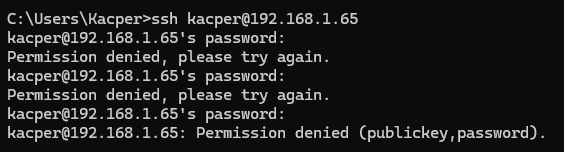
\includegraphics[width=0.97\textwidth]{images/nouser1}}
  \caption[Incorrect Credentials]{Incorrect Credentials - user 'kacper'}\label{fig:noUser1}
\end{figure}

\begin{figure}[!h]
  \centering
  \fbox{\rule{0pt}{3.5cm}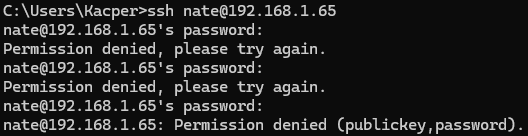
\includegraphics[width=0.97\textwidth]{images/nouser2}}
  \caption[Incorrect Credentials]{Incorrect Credentials - user 'nate'}\label{fig:noUser2}
\end{figure}

As the users are not able to access the \gls{ssh} terminal with incorrect credentials, the test is given a pass.

\section{Discussion}\label{sec:discussion}
% Critical appraisal: strengths, weaknesses, methodology choices; comparison
% with prior work. Optional: ablation analysis, sensitivity analysis.
This section will address the strengths and weaknesses of the proposed solution, highlighting methodological choices and why they were chosen along the way.

\subsection{Strengths}\label{subsec:strengths}
The proposed solution throughout was testing was largely successful. One of the key strengths that helped contribute to the systems success was reliably being able to connect to the system remotely. As demonstrated through testing, the system is able to be interfaced with and managed entirely remotely, with no necessary physical interaction. The commands sent through the remote interface are fast and execute all the necessary actions a media player requires. The remote solution is also not limited to just a Command Line Interface, as users are able to connect using \gls{vnc} if they prefer a graphical interface. This directly addresses the main objective of the remote management for the system and through testing, it is strongly suggested that the system is efficient with its remote communication.

Simplicity in its physical implementation strengths the belief the system is successful. As backed by research conducted in section \ref{subsec:medContext} and the informal chat with ENRICH Cymru, this was the most important aspect of the implementation. The system provides a simple \gls{ui} through its remote solution, but omits one through its hardware, presenting only two simple buttons to perform two simple actions. Avoiding over-complicating the device ensured that the main stakeholders were still the focus throughout development, creating a truly tailored solution for the cognitively impaired.

Finally, the system addresses an important aspect of life that may be missed in assistive technologies for the cognitively impaired, especially patients with dementia. The neglect of making leisure accessible is apparent, considering the positive impact that it has on the mental wellbeing of dementia patients. The focus on delivering music in an accessible manner tackles this unexplored market of accessible technologies and provides a proof of concept that technology can be designed with accessibility embedded in its development. This is a strength as it highlights a disparity within the field of assistive technologies focusing mostly on care and extending 'quantity of life', rather than 'quality of life'.  

\subsection{Weaknesses}\label{subsec:weaknesses}
The proposed solution is not without its flaws. For instance, although the system is intended to run completely offline, it does require a constant internet connection to be able to interface with it remotely, either through \gls{ssh} or \gls{vnc}. The alternative would be to manage the system offline but this would require a constant keyboard, mouse and monitor to be connected to the device. This could be mitigated if given more time and resources but the current state of the proposed solution requires a constant internet connection.

Being a device tailored towards simplicty, the inital setup of the device is complex and does require a level of technical knowledge to enact. Should the proposed solution come packaged with the correct prerequisites, a mouse, keyboard and monitor are still required to ensure that the device can be connected to a new network to enable remote management. Connection to this new network then imposes its own \gls{dhcp} protocol onto the proposed solution and assigns it a new IP address. Even if a static IP address was assigned beforehand, there is no guarantee that the IP address hasn't already been taken by another device or if the device used to \gls{ssh} onto the proposed solution is in the same subnet and can contact the proposed solution. This could as well be mitigated if given more time and resources.

Finally, \gls{nfc}, one of the main features and methods of interaction, requires a level of setup that isn't intuitive. This is primarily due to a lack of testing on alternatives, however, there only exists one supported way of writing to the \gls{nfc} tags. The script on the Arduino must be switched to an alternative writing script and then switched back to the reading script before the \gls{nfc} functionality is restored to the proposed solution. The switching of the scripts requires a separate device that has access to the Arduino IDE and the accompanying Arduino library that contains the functionality to interface with PN532 devices, that being the \gls{nfc} module. This would have to occur each time a new playlist (or if the playlist is to be shuffled or not) has been added to the proposed solution if the user wishes for all the playlists to be available using \gls{nfc}. This undermines the simplicity of the device if such intricate setup processes are necessary beforehand. 

\subsection{Methodology Choices}\label{subsec:methodology}
The project was completed utilising a Waterfall Methodology throughout its development. This was set out by the inital plan that was completed prior to the start of this project, where clear deliverables were identified and milestones generated. Each feature was developed in a vacuum week by week in its entirety until it was integrated into the system at large. This methodology did remain flexible to allow for buffers between features if development took longer than expected or bugs were identified within the modules.

The predictability within the Waterfall Model was beneficial as it helped keep discussions with the project supervisor directed, it ensured that each week quantifiable progress can be observed and time could be effectively managed based on progress as each feature was given a predetermined time slot that was open for alteration.

\chapter{Conclusions and Future Work}\label{ch5}
% =============================================================================
% CHAPTER 5: Conclusions and Future Work
% =============================================================================
% SPDX-FileCopyrightText: 2026 Frank Langbein <frank@langbein.org>
% SPDX-License-Identifier: LPPL-1.3c
%
% Suggested sections: Conclusions; Future work. Do not introduce new material in
% Conclusions---summarise aims and main results. Future work: next steps, open
% questions, what you would do with more time. Optional: short summary of
% contributions (as part of Conclusions or a bullet list).
% =============================================================================

This chapter concludes the dissertation. Summarise the aims, main results, and what was learned; then outline future work and improvements.

\lipsum[35-36]

\section{Conclusions}\label{sec:conclusions}
% Summary of aims, key results, and main takeaways. Optional: list of contributions.

% Terminal Interaction
Based off these results, we can conclude that each command that is passed into the terminal returns the expected output, satisfying Functional Requirement \ref{req:correctCommand}.

% Button Interaction
Based off these results, it can be concluded that the proposed solution can be interfaced with using button interaction, satisfying Functional Requirements \ref{req:playBtn} and \ref{req:skipBtn}. 

% load_playlist
This demonstrated the robustness of the module, its tolerance for different types of inputs and its functionality working as intended. These unit tests are not attributed to any particular Functional Requirement but feed into ensuring that the system as a whole is working as intended.

% NFC
satisfied \ref{req:NFCcorrect} and \ref{req:NFCtolerance}

% Response Time
satisfied \ref{req:reboot}, \ref{req:remoteTime}, \ref{req:startupTIme}, \ref{req:usable}

% Misc Tests
satisfied \ref{req:scalability}, \ref{req:remoteAuth}, \ref{req:audioPlayback}, \ref{req:remoteCon}

\lipsum[37-38]

\section{Future work}\label{sec:future}
% Next steps, open questions, and what you would do with more time or resources.
satisfy \ref{req:easeofuse}

\lipsum[39-40]


\chapter{Reflection on Learning}\label{ch6}
% =============================================================================
% CHAPTER 6: Reflection on Learning
% =============================================================================
% SPDX-FileCopyrightText: 2026 Frank Langbein <frank@langbein.org>
% SPDX-License-Identifier: LPPL-1.3c
%
% Suggested sections: Critical narrative of the experience; Analysis and application;
% Implications for future practice. Focus on transferable learning and (where
% applicable) ``double loop learning'': impact on assumptions and concepts, not
% only skills. Optional alternatives: ``What I would do differently''; ``Transferable
% skills and concepts''. Omit this chapter if not required by your institution;
% comment out the \chapter and \input in main.tex.
% =============================================================================

\newthought{Committing to a project} of this caliber and the time to focus a majority of the Author's time to it has provided some critical reflections for the Author about the project as a whole and how they learn independently.

\section{Critical narrative of the experience}\label{sec:challenges}
% Key challenges, turning points, and how they affected your understanding.
Producing a solution tailored for an end user that is not the Author was a learning experience. Most of the applications that the Author created beforehand have been either coursework assignments or simple programs that the Author could always amend. This encouraged the Author to produce as cohesive and as self-sufficient of a product as possible. The Author encountered a variety of challenges and would like to highlight some of them and what they learnt from them.
\begin{itemize}
    \item \textbf{Working with Embedded Systems} - Specialised hardware is designed for a specific purpose and has specific requirements for it to work alongside the system as a whole. The Author acknowledged that many of these requirements may not be obvious at first so prior research into the embedded systems and their components is vital. This can be seen in the OS incompatibility with the GrovePi+ shield for the Raspberry Pi. The surface level information the Author was provided with was insufficient as it was the further research that made them realise the kernel incompatibility and deprecated URLs for certain packages. This highlighted the importance of research that cannot be overstated, which the Author will take into consideration from this point forward.  
    \item \textbf{Planning for the Long-Term} - Working with different parties and stakeholders within a project naturally creates trouble in terms of scheduling, which the Author did not fully grasp. The Author left it too late for any ethical application to be sent off in time and then arrange for user testing, which should have happened during the beginning of the project to ensure the possibility of user testing. This can also be reflected in more continuous contact with the project supervisor. Had the Author engaged with the supervisor more, they could have potentially identified the need for ethical approval for user testing much sooner and reached out to more researchers to obtain their feedback on the proposed solution, helping direct development with clear tailored objectives for the proposed solution, rather than what the Author assumed would be suitable.
\end{itemize}

Ultimately, the Author has learnt a lot about how a development pipeline with weekly meetings would work. The Author now knows how to appropriately plan for potential hardship within a project and when to ask for help when it is necessary. The Author learnt how to do more targeted research and how to find basis or possible disputes in the assumptions that the Author may have previously had. Finally, the Author learnt how to engage with the public on a piece of research and how to communicate effectively with their colleagues to boost the productivity of their research into a solution.



\backmatter

% -----------------------------------------------------------------------------
% Appendices (lettered A, B, ... in headers and TOC)
% -----------------------------------------------------------------------------
\appendix
\chapter{Supplementary Material}\label{app:supp}
\input{Appendix/appendix}

% Bibliography (always last): \bib{bibfile} uses natbib (numeric or harvard per class option)
% and inserts the License chapter if \license was set.
\bib{bibliography}

\end{document}
